\section{Микросервисы}

Микросервисы — это архитектурный подход к разработке программного обеспечения, при котором приложение состоит из небольших независимых сервисов, взаимодействующих через чётко определённые API. 

Архитектура микросервисов упрощает масштабирование приложений и ускоряет их разработку, что способствует инновациям и сокращает время вывода новых функций на рынок.


Микросервисы имеют ряд преимуществ:
\begin{enumerate}[label=\arabic*)]

   \item \textbf{Более эффективное использование ресурсов}.
Микросервисная архитектура позволяет гибко подгонять каждый сервис под конкретную нагрузку. Оптимально распределяя вычислительные ресурсы, можно добиться лучшего коэффициента их использования и грамотного масштабирования.

Например, сервису с высоким CPU-потреблением выделяют больше вычислительных ядер, тогда как сервису, которому критичен объём памяти, — больше RAM.

Такая оптимизация снижает операционные затраты приложения и повышает общую эффективность работы системы.

     \item  \textbf{Гибкое масштабирование (Flexible Scaling)}.	 Каждый сервис можно масштабировать независимо, ориентируясь на нагрузку именно той функции, которую он обеспечивает. Это позволяет точно подбирать ресурсы, понимать стоимость конкретной фичи и сохранять доступность при всплесках трафика.
   \item \textbf{Простота деплоя (Easy Deployment)	}.Микросервисы облегчают CI/CD: пробовать новые идеи и откатываться при неудаче становится дешевле. Низкая цена ошибки поощряет эксперименты и ускоряет вывод новых возможностей на рынок.
   \item \textbf{Изоляция отказов}.
Когда какой-либо сервис в микросервисной архитектуре выходит из строя, остальная система продолжает работать, поскольку каждый сервис функционирует независимо. Такая изоляция отказов повышает надёжность всей системы и облегчает разработчикам поиск и устранение неисправностей: понятно, какой именно сервис «болит».


\end{enumerate}


\begin{figure}[H]
    \centering
    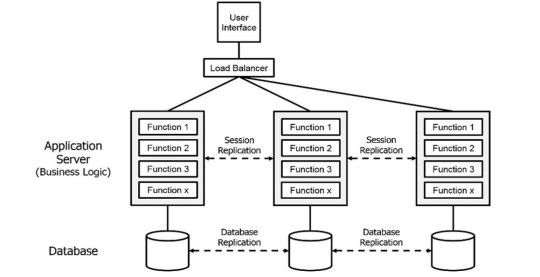
\includegraphics[width=0.7\textwidth]{styles/diploma/inc/microservice1.png} 
    \caption{Пример микросервисной архитектуры. На рисунке видно, как каждый сервис полностью независим от других сервисов.}
    \label{fig:example}
\end{figure}

Таким образом, в системе заложены ключевые принципы — изоляция отказов, гибкое масштабирование и эффективное использование ресурсов. Следующий шаг — организовать надёжное взаимодействие между микросервисами.

В выбранной архитектуре один сервис отвечает за бизнес-логику приложения, а другой — за инференс модели. Чтобы модель своевременно получала новые данные, необходим асинхронный канал обмена сообщениями. Оптимальным решением здесь становится очередь RabbitMQ



